\section{Results}
\label{sec:results}

\subsection{Adoption of \gls{DMARC} in different countries}
\begin{table}[tb]
\footnotesize
\centering
\caption{Top ccTLD countries by DMARC adoption, policy types, and total domains with stringent policies.}
\begin{tabular}{lrrr}
\toprule
\textbf{Country} & \textbf{All} & \textbf{Policies (\%)} & \textbf{Stringent} \\
\midrule
Germany & 8.9M & 2.5M (27.9\%) & 1.5M (60.0\%) \\
Netherlands & 3.4M & 1.9M (56.1\%) & 861.1k (45.4\%) \\
United Kingdom & 6.5M & 1.3M (20.3\%) & 518.8k (39.7\%) \\
Italy & 2.2M & 1.0M (45.4\%) & 81.3k (8.1\%) \\
Brazil & 3.4M & 950.5k (27.7\%) & 143.3k (15.1\%) \\
Poland & 1.8M & 884.9k (50.0\%) & 426.5k (48.2\%) \\
France & 2.7M & 790.1k (29.2\%) & 276.1k (34.9\%) \\
Australia & 2.7M & 642.1k (23.6\%) & 246.1k (38.3\%) \\
Switzerland & 1.5M & 610.1k (40.2\%) & 426.6k (69.9\%) \\
India & 2.6M & 587.0k (22.7\%) & 272.6k (46.4\%) \\
\bottomrule
\end{tabular}
\label{tab:dmarc_country_policies}
\vspace{-15px}
\end{table}
We summarize the top countries by total number of domains with \gls{DMARC} in~\cref{tab:dmarc_country_policies}.
We observe a skewed distribution with a few countries leading the adoption of \gls{DMARC}.
For instance, Germany (top of the list) has 4.3$\times$ more adoption than India (last in our list) (2.5M domains with \gls{DMARC} vs. 587k).
Out of all countries we measured \gls{DMARC}, the top 23 represent 80\% of global \gls{DMARC} adoption.
However, only the Netherlands has more than 1.9M (50\%) of its domains configured \gls{DMARC} from the top 10 adopters, with the UK the lowest in relative terms (1.3M, 20.3\%).

Using our categories of stringent and permissive policies, we observe uneven distribution of stringent policies by the top countries, ranging from 8.1\% (81.3k) in Italy to 69.9\% (426.1k) in Switzerland.
Italy and Brazil stand out as countries with high \gls{DMARC} adoption but low levels of stringent policy use.
Italy's guidelines to use \gls{DMARC} are recent (August 2025)~\cite{_FrameworkDiAutenticazione_}, so we can speculate that domain owners are still in the process of moving from monitoring to enforcement.
Brazil CERT's recommendation is rather superficial, mentioning \gls{DMARC} and its relevant RFC but without providing instructions and a rollout plan~\cite{RECOMENDACAO172023_}.
Germany and Switzerland stand out as top adopters, with a better stringent-permissive policy ratio.
Germany has a clear national technical guideline on \gls{DMARC} dated January 2024~\cite{_BSITR03182Email_}, which specifies what email providers must do to verify \gls{DMARC} records and domains sending email that must implement \gls{DMARC}.
The Swiss registry ``Switch'' has a financial incentive to adopt \gls{DMARC} starting in 2024, as mentioned in their 2023 report~\cite{_Report2023Ch_}.

\iffalse
\begin{figure}[ht]
    \centering
    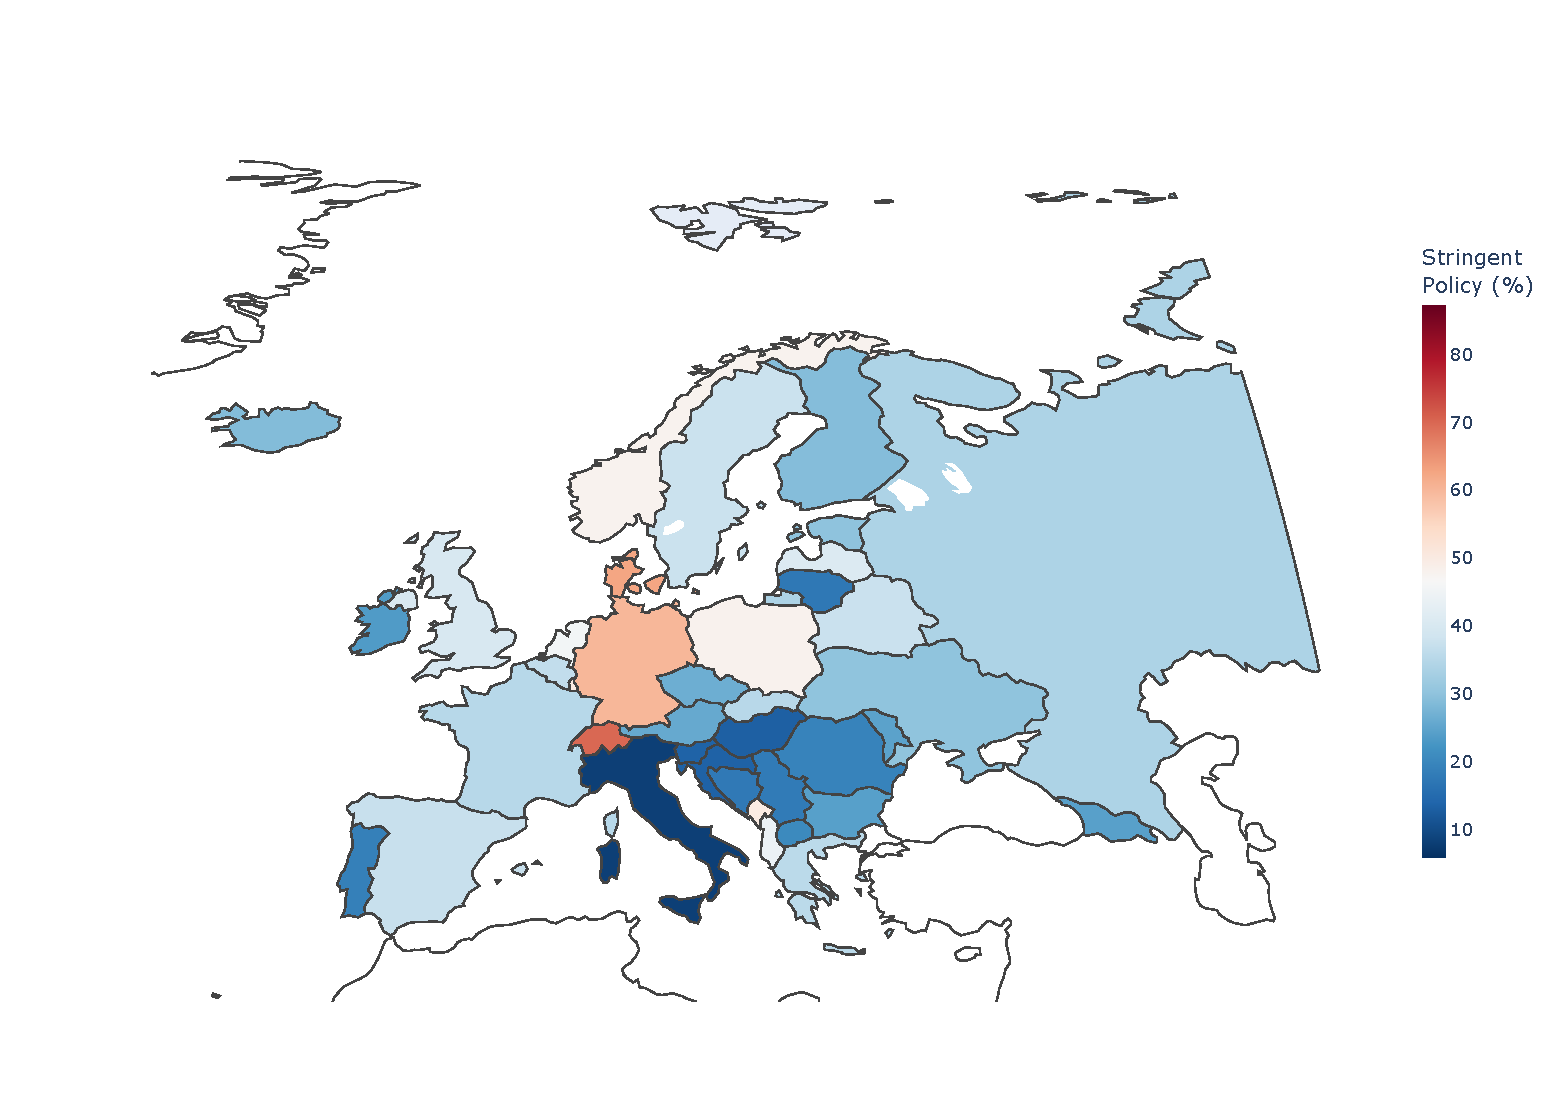
\includegraphics[width=\linewidth]{figures/europe_map_stringent_policy_percentage.pdf}
    \caption{DMARC policies adoption in Europe.}
    \label{fig:europe_map_policy}
\end{figure}

\begin{figure}[ht]
    \centering
    \begin{subfigure}{0.47\textwidth}
        \centering
        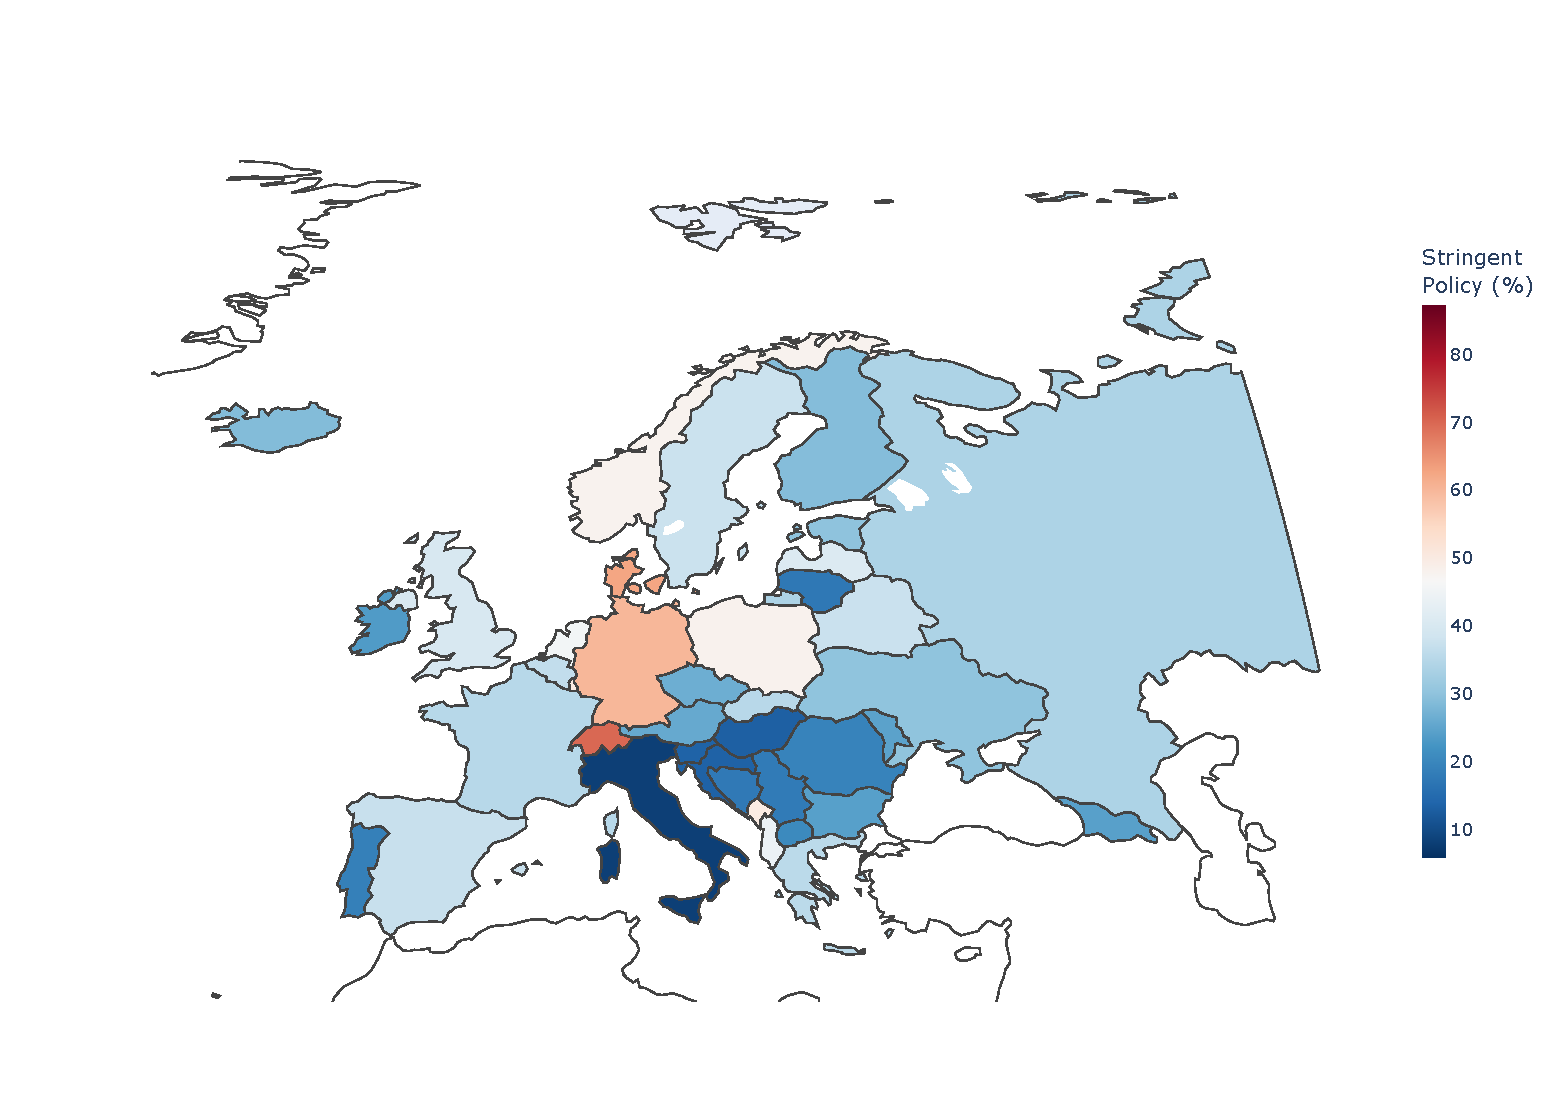
\includegraphics[width=\linewidth]{figures/europe_map_stringent_policy_percentage.pdf}
        \caption{All ccTLDs.}
        \label{fig:world_map_policy}
    \end{subfigure}
    \hfill
    \begin{subfigure}{0.49\textwidth}
        \centering
        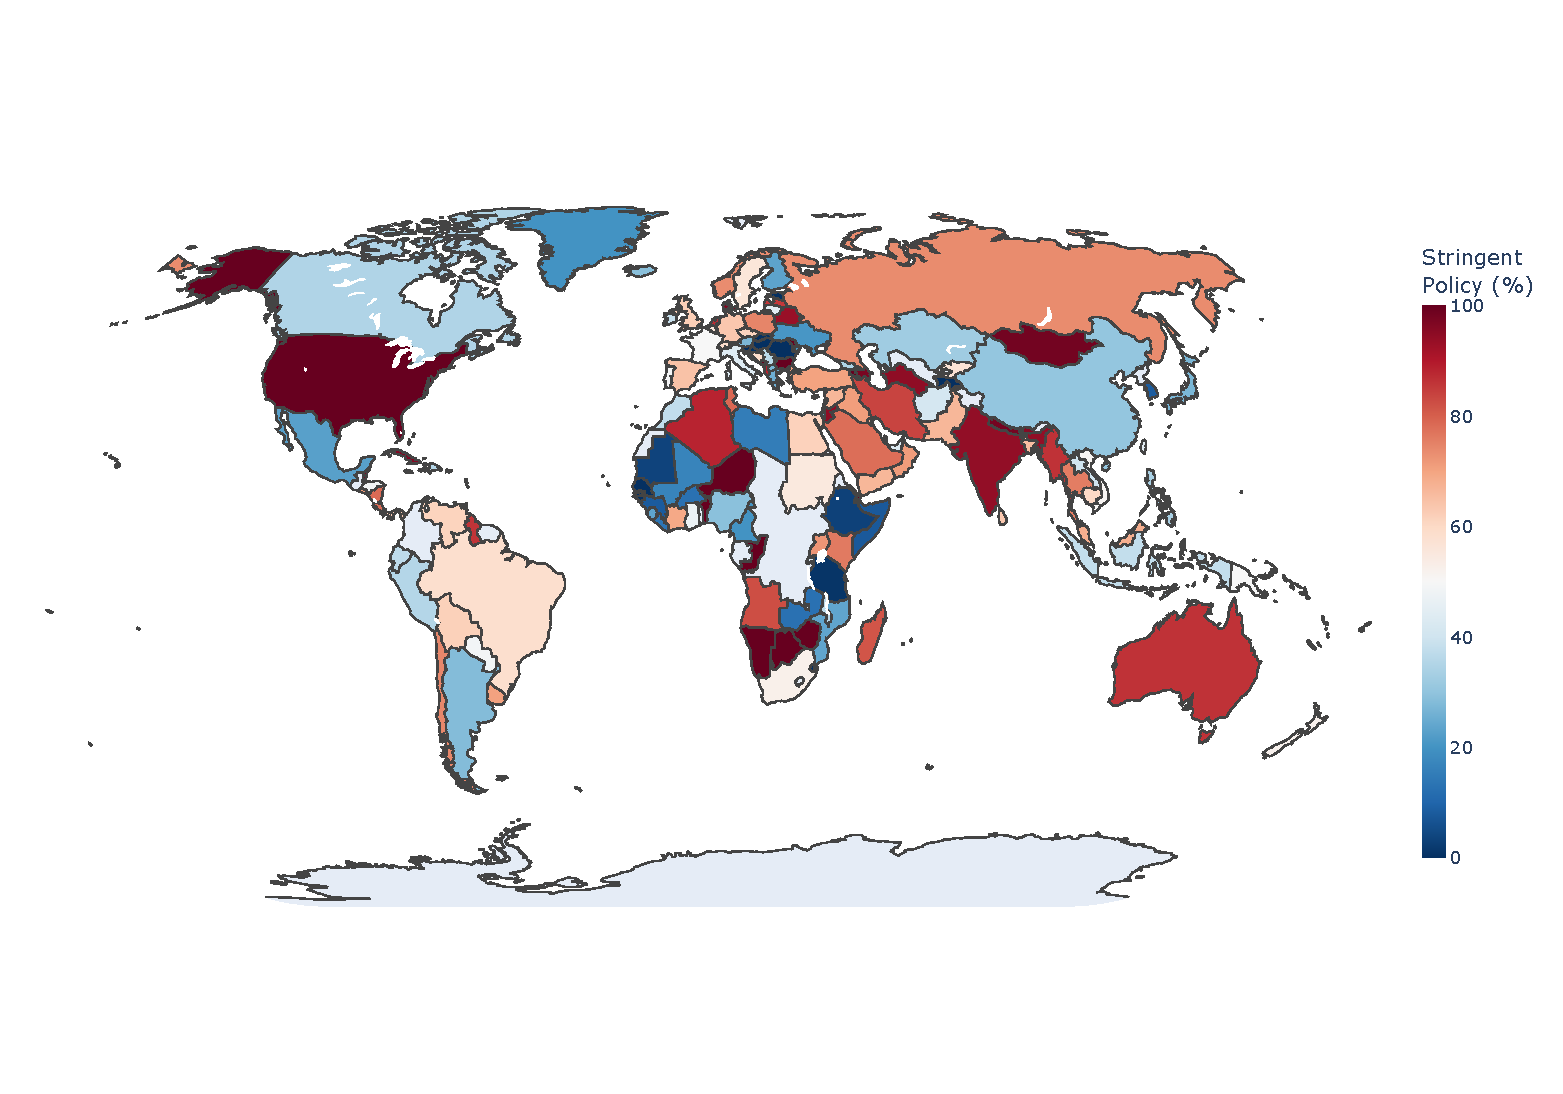
\includegraphics[width=\linewidth]{figures/gov_world_map_stringent_policy_percentage.pdf}
        \caption{Governmental domains.}
        \label{fig:gov_world_map_policy}
    \end{subfigure}
    \caption{Categories of DMARC policy ratio worldwide. 
    (a) Across all ccTLDs. (b) Across government domains.}
    \label{fig:world_map_policy_subfigures}
\end{figure}
\fi

We observe that Europe has the highest \gls{DMARC} usage, with 12.3M domains (30\%). However, 34.5\% (5.2M) of its domains use stringent policies, only in front of Africa, in percentage terms, with 33\% (145.1k) and less than North America, which leads with 50\% (457.0k). From Europe's perspective, CERT-EU issued recommendations in 2017 to combat email abuse using \gls{DMARC}~\cite{Koutroumpas_EUDirectiveDMARC_}. However, we observe that more effort is needed to improve European domain names' adoption of \gls{DMARC} stringent policies.

We perform a longitudinal analysis of \gls{DMARC} policies, from February 2024 to October 2024, using \openintel historical data. It is worth noting that a few countries are missing a longitudinal measurement point. However, this does not significantly affect our analysis, as we still observe the overall trends.
The only exception is a sharp rise in French domains (FRA) in February 2025, which is due to an artefact in the \openintel-provided \texttt{.fr} data.
We selected the countries that adopt \gls{DMARC} the most during this period. The~\cref{fig:longitudinal_analysis} shows the domain counts per policy (\texttt{none, quarantine} and \texttt{reject}) alongside the total number of domains per country.
Surprisingly, we found Colombia in our top adopters. We could not find relevant documentation in Colombian sources. Hence, we can at best speculate that \texttt{.co} is used for purposes beyond regional Colombian content~\cite{_DominioCO_}, with Google classifying it as a generic \gls{ccTLD}~\cite{_ManagingMultiRegionalMultilingual_a}.
The clear guidelines from Germany and incentives from the Swiss registry contributed to the gradual increase in adoption of \gls{DMARC}, with transition to more stringent policies (\eg \texttt{reject}).
The Netherlands also follows this trend. We observe that the Dutch registry endorses the German guidelines~\cite{_GermanysBSIPublishes_}.
On the contrary, Brazil and Italy show low numbers of stringent policies in the short span of our analysis. We correlate with their previously mentioned national strategies, which lack \gls{DMARC} policy rollout plans.

\begin{figure}[tb]
    \centering
    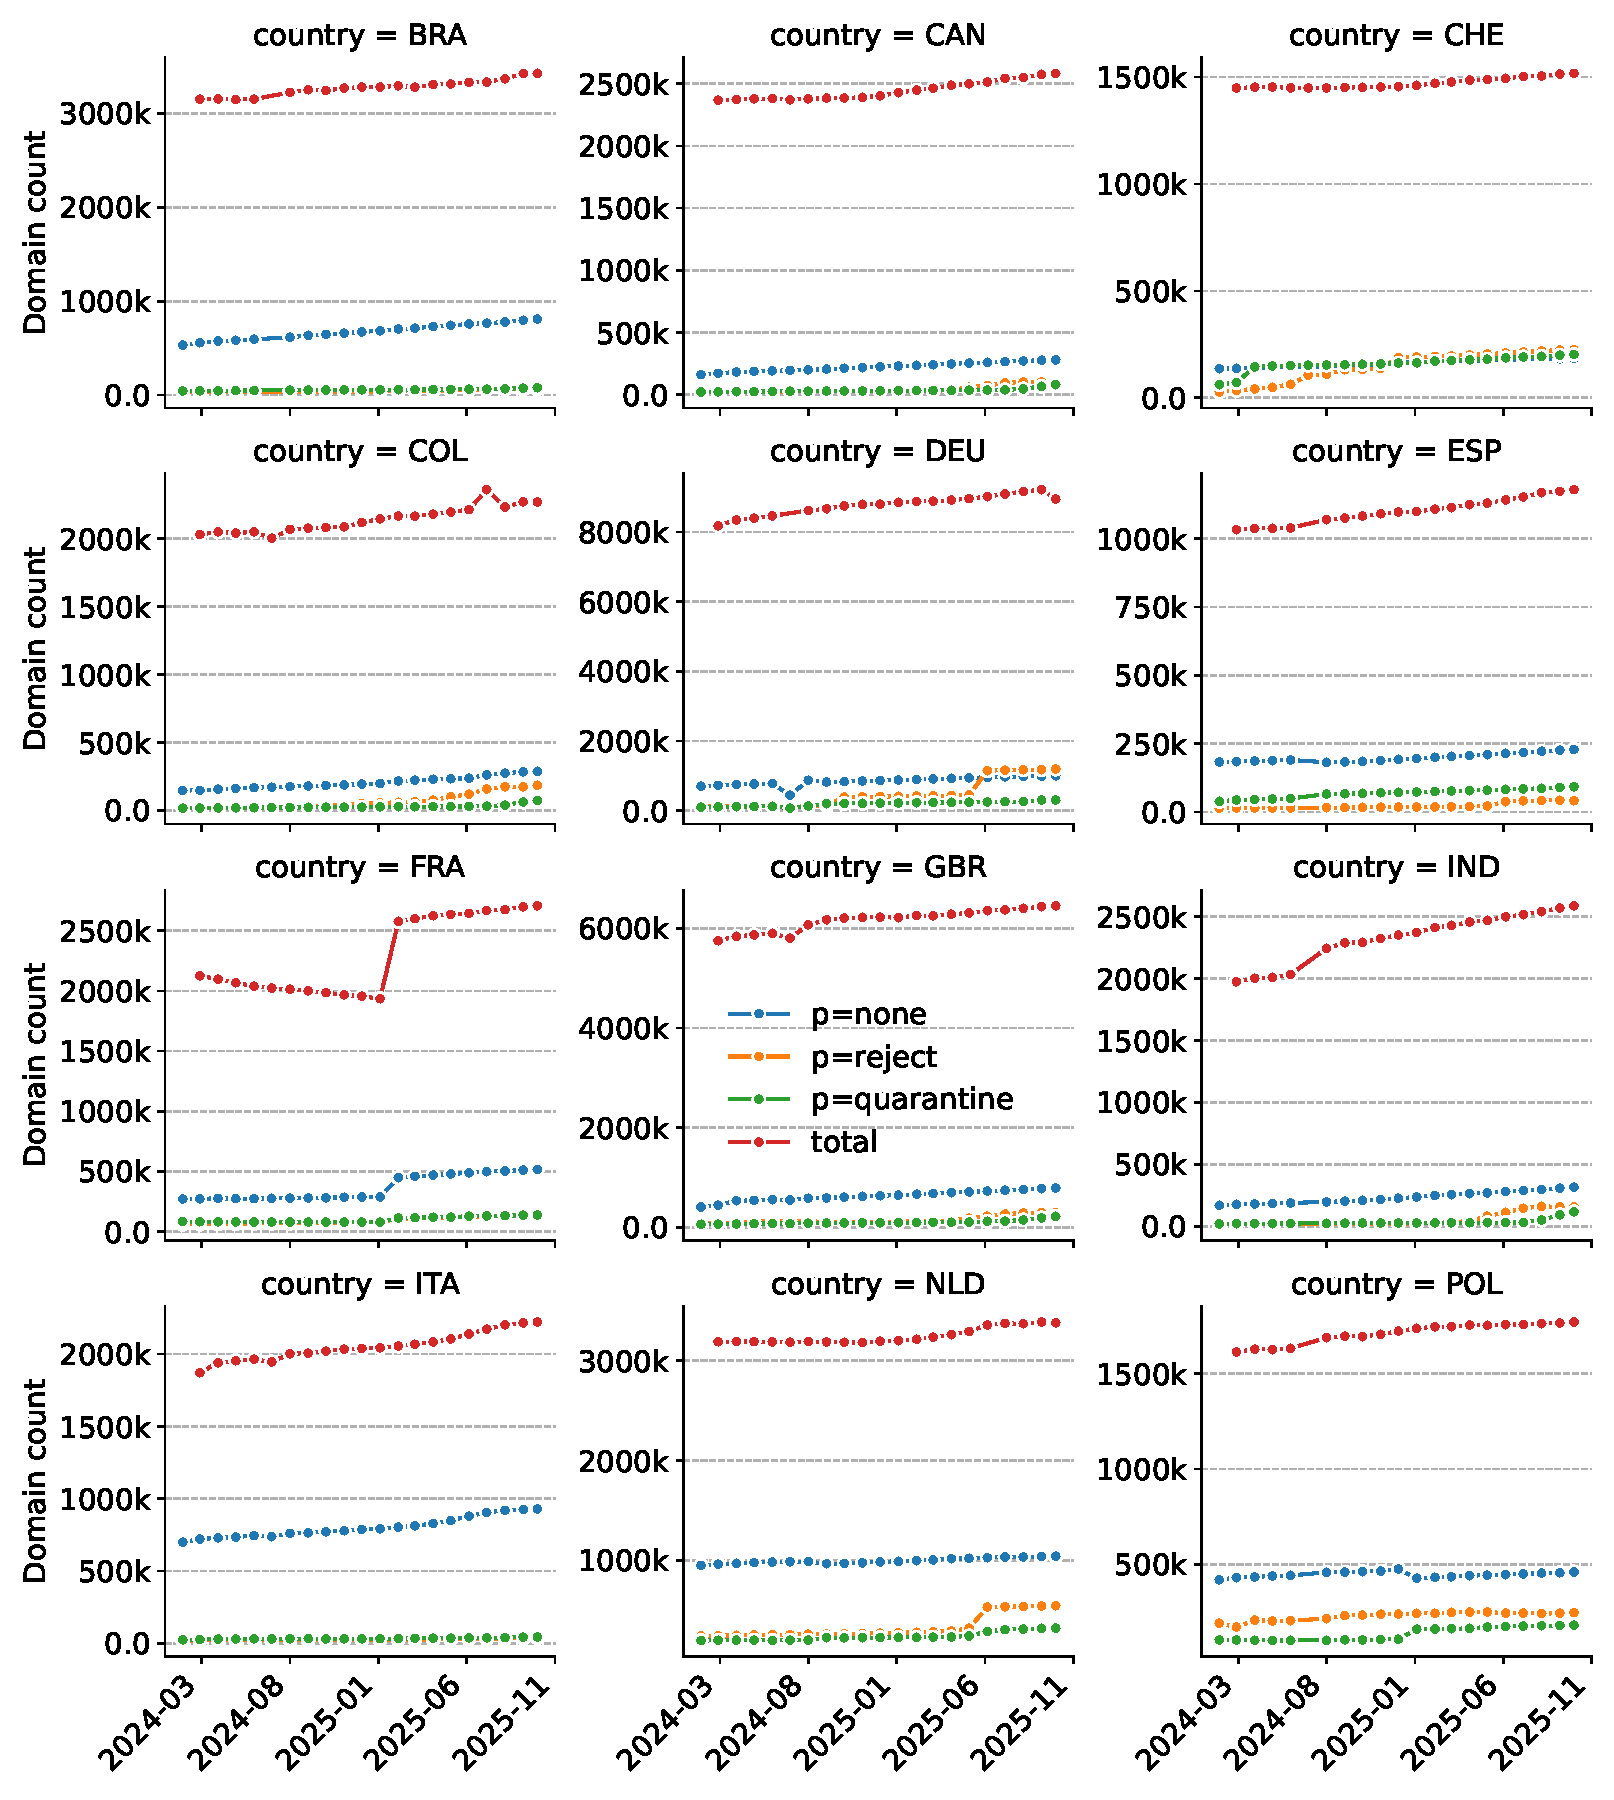
\includegraphics[width=1.\linewidth]{figures/longitudinal_analysis.pdf}
    \caption{Longitudinal analysis of countries that adopt the most DMARC, from 2024-02 to 2025-10.}
    \label{fig:longitudinal_analysis}
    \vspace{-20px}
\end{figure}

\textbf{DMARC policies in government domains.}
\begin{table}[tb]
\centering
\scriptsize
\caption{Top countries by DMARC adoption among government domains.}
\label{tab:gov_dmarc_country}
\begin{tabular}{lrrr}
\toprule
\textbf{Country} & \textbf{All} & \textbf{Policies} & \textbf{Stringent}\\
\midrule
United Kingdom & 6.5M & 4.7k & 2.9k (62.2\%) \\
Thailand & 86.3k & 2.7k & 2.1k (75.8\%) \\
India & 2.6M & 2.4k & 2.2k (94.3\%) \\
Mexico & 718.3k & 1.6k & 356 (22.7\%) \\
Argentina & 408.4k & 1.5k & 420 (28.2\%) \\
Ukraine & 335.5k & 1.4k & 285 (20.7\%) \\
Indonesia & 682.7k & 991 & 374 (37.7\%) \\
Türkiye & 498.3k & 983 & 691 (70.3\%) \\
Switzerland & 1.5M & 975 & 573.0 (58.8\%) \\
Ecuador & 33.2k & 930 & 344 (37.0\%) \\
%Australia & 2.7M & 834 & 721 (86.5\%) \\
\bottomrule
\end{tabular}
\vspace{-15px}
\end{table}

We summarize the countries with the most government domains that adopt \gls{DMARC} in~\cref{tab:gov_dmarc_country}, and the adoption of stringency policies per country. The United Kingdom leads as the most adopter. There has been a clear UK government guideline to use \gls{DMARC}~\cite{_SecuringGovernmentEmail_2024} since 2016. It is surprising that, despite such early advisory notification, only 2.9k (62.2\%) of government domains have stringent policies.
India has the highest adoption rate of strict \gls{DMARC} policies among government domains (2.2k, 94.3\%). The mandatory security guidelines issued by CERT-In require government entities to comply with specific cybersecurity measures--including the use of \gls{DMARC}~\cite{Awasya_GuidelinesInformationSecurity_}.
Mexico has a poor ratio of government domains with stringent \gls{DMARC} policies. We could not find any information on Mexico's government about \gls{DMARC} strategies~\cite{mexico_ciberseguridad}.
Similar to \gls{ccTLD} domains, we find a skewed distribution of government domains using \gls{DMARC}. Of the 183 countries, 42 account for 80\% of all government domains. We summarize the top governments that adopt \gls{DMARC} in~\cref{tab:gov_dmarc_country}.

~\cref{fig:stringent_vs_permissive_policies_correlation} shows the correlation between stringent and permissive policies among domain names under \gls{ccTLD}.
We observe Germany, Switzerland, Italy, and Brazil as outliers. However, we see that domains from \glspl{ccTLD} tend to have more permissive policies than stringent ones.
This scenario changes when we analyze government domains.~\cref{fig:gov_stringent_vs_permissive_policies_correlation} shows that government domain names under many \glspl{ccTLD} tend to have stringent rather than permissive policies.

\begin{figure}[tb]
    \centering
    \begin{subfigure}{0.24\textwidth}
    %\begin{subfigure}{0.35\textwidth}
        \centering
        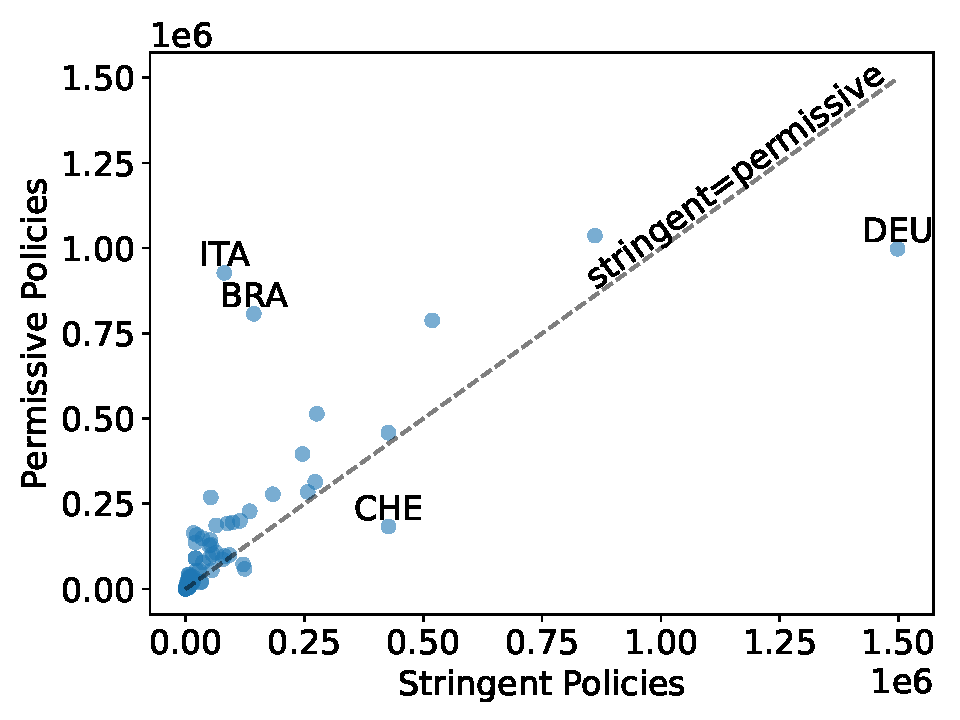
\includegraphics[width=\linewidth]{figures/stringent_vs_permissive_policies_correlation.pdf}
        \caption{ccTLD domains.}
        \label{fig:stringent_vs_permissive_policies_correlation}
    \end{subfigure}
    \hfill
    \begin{subfigure}{0.24\textwidth}
        \centering
        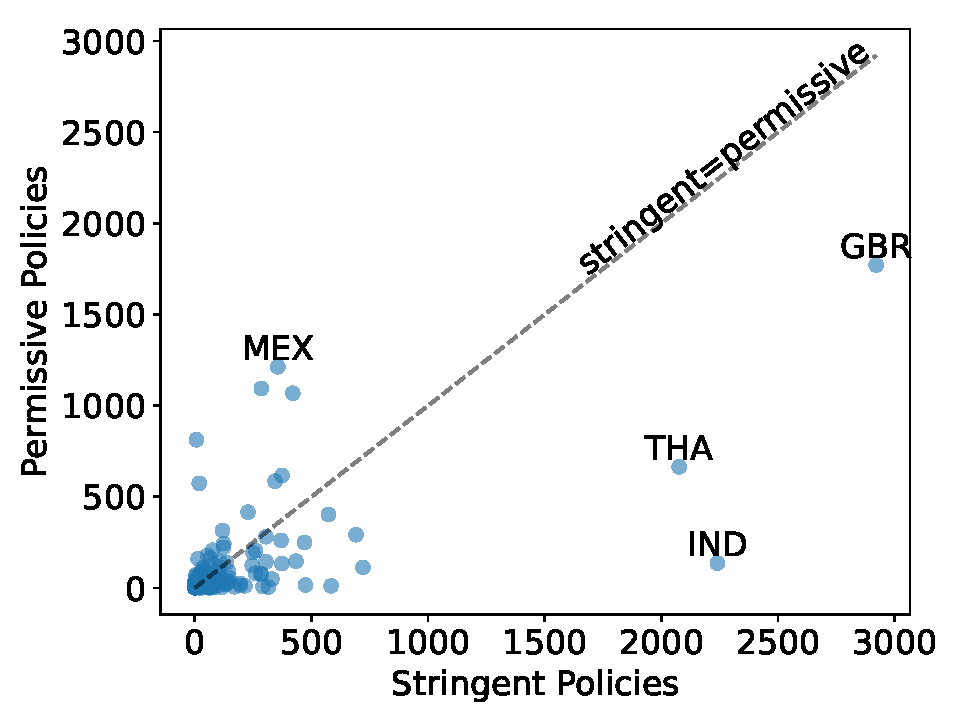
\includegraphics[width=\linewidth]{figures/gov_stringent_vs_permissive_policies_correlation.pdf}
        \caption{Government domains.}
        \label{fig:gov_stringent_vs_permissive_policies_correlation}
    \end{subfigure}
    \caption{Correlation of DMARC policies.}
    \label{fig:correlation_subfigures}
    \vspace{-15px}
\end{figure}

We observe a steady increase in \gls{DMARC} adoption across most of the top countries in government domains over time. Notably, the United Kingdom and Switzerland show increased policy use, indicating both an increase in adoption over time and a rollout strategy toward more stringent policies~\cite{_6ContinuousImprovement_,_Report2023Ch_}.
India is one of the few countries where \gls{DMARC} adoption has not grown. However, it maintains a high percentage of stringent policies throughout the period analyzed, demonstrating the effectiveness of its national guidelines.

\subsection{The landscape of \gls{DMARC} reporting}
Compared to prior work~\cite{hureau_spoofed}, we observe a few notable changes in the top reporting centers. For instance, we see a reduction in private mailbox (Gmail) from 1.28\% to 0.8\% (50.7k).
% it's tricky to get the absolute number right from prior work because they report percentages and I don't from which total number (11.7M or 4.0M, I GUESS the latter): "Over 6.8 M domain name owners have expressed interest in receiving at least one type of reports, with a combined total of 11.7 M email addresses, 4.0 M of which are unique"
Specialized email security companies, such as Proofpoint, Agari, and MailinBlue, appear less, from 14.42\%, 3.04\%, and 3.78\% to 1.5\% (96.3k), 0.5\% (34.0k), and 0.6\% (36.2k), respectively.
There is an increase in hosting organizations receiving \gls{DMARC} reports. We find \textit{onsecureserver.net} (19.3\%, 1.2M) tops our list (associated with GoDaddy~\cite{_GoDaddyWatDKIM_}).
Starting from April 2025, domains obtained through GoDaddy have \gls{DMARC} reports sent to onsecureserver.net by default.
Cloudflare has a higher share, from 1.58\% to 4.5\% (282.1k), and simply.com appears in our top 10 (1.2\%, 73.4k).

\begin{table*}[ht]
  \centering
  \scriptsize
  \caption{Top reporting countries and their top report receiver domain.}
  \begin{subtable}[t]{0.3\textwidth}
    \scriptsize
    \centering
    \caption{All ccTLD domains}
    \label{tab:top10_reporting_country}
    \begin{tabular}{lrrr|}
    \toprule
    & \textbf{All} & \textbf{Pol.→Reporting (\%)} & \textbf{Top report receiver} \\
    \midrule
    United Kingdom & 6.5M & 1.3M (20.3\%) → 43.0 & onsecureserver.net (38.1\%) \\
    Netherlands & 3.4M & 1.9M (56.1\%) → 22.1 & reportdmarc.nl (34.6\%) \\
    Germany & 8.9M & 2.5M (27.9\%) → 15.0 & dmarc.brevo.com (7.0\%) \\
    Colombia & 2.3M & 541.7k (23.9\%) → 61.3 & onsecureserver.net (26.7\%) \\
    Australia & 2.7M & 642.1k (23.6\%) → 47.4 & onsecureserver.net (29.3\%) \\
    India & 2.6M & 586.9k (22.7\%) → 48.3 & onsecureserver.net (75.1\%) \\
    Poland & 1.8M & 884.9k (50.0\%) → 31.5 & lh.pl (21.6\%) \\
    Brazil & 3.4M & 950.3k (27.7\%) → 25.0 & onsecureserver.net (12.2\%) \\
    Canada & 2.6M & 461.6k (17.9\%) → 47.8 & onsecureserver.net (44.1\%) \\
    France & 2.7M & 790.1k (29.2\%) → 23.9 & dmarc.brevo.com (20.2\%) \\
    \bottomrule
    \end{tabular}
  \end{subtable}
  \hfill
  \begin{subtable}[t]{0.5\textwidth}
    \scriptsize
    \centering
    \caption{Governmental domains}
    \label{tab:gov_top_reporting_countries_and_top_report_receiver}
    \begin{tabular}{lrr}
    \toprule
    & \textbf{Pol.→Reporting (\%)} & \textbf{Top report receiver} \\
    \midrule
    United Kingdom & 4.7k → 61.7  & dmarc.service.gov.uk (50.9\%) \\
    Tanzania       & 820 → 99.9   & gov.go.tz (56.6\%) \\
    Australia      & 834 → 90.9   & vali.email (8.6\%) \\
    Thailand       & 2.7k → 24.8  & sukplus.com (5.0\%) \\
    Argentina      & 1.5k → 44.4  & dmarc-reports.cloudflare.net (6.1\%) \\
    Nepal          & 595 → 99.5   & nitc.gov.np (97.5\%) \\
    New Zealand    & 586 → 93.0   & inbox.ondmarc.com (10.0\%) \\
    Bangladesh     & 719 → 71.3   & ruf.dmp.cisco.com (34.6\%) \\
    Mexico         & 1.6k → 32.2  & transparenciasonora.gob.mx (5.9\%) \\
    India          & 2.4k → 21.2  & ardhas.com (2.1\%) \\
    \bottomrule
    \end{tabular}
  \end{subtable}
  \label{tab:combined_top_reporting_countries_and_top_report_receiver}
  \vspace{-15px}
\end{table*}

~\cref{tab:top10_reporting_country} shows the top countries that send \gls{DMARC} reports.
For each country, we provide the total number of domains and the number of domains with \gls{DMARC} policies (and their percentage of the total domains). Following, the percentage of domains reporting, relative to domains with \gls{DMARC}, the top reporting receiver, and its share among other reporting receivers for that country.
We observe that Germany has the lowest adoption of \gls{DMARC} reporting, with only 373.6k (15\%). Although Germany leads in total number of domains (2.5M domains), our evidence suggests that domain owners are not following the practices advised by Germany's Federal Office for Information Security~\cite{_BSITR03182Email_}.
Colombia has the highest percentage of domains that configured \gls{DMARC} reporting (332.1k, 61.3\%).
It has 13\% more than the second, India (283.6k, 48.3\%).
%Due to a lack of documentation, we speculate that the \texttt{.co} domain might be used by organizations outside Colombia, which could affect our analysis.

In general, U.S.-based \gls{DMARC} report receivers lead with 1.8M (26.7\%) domains. The top report-receiving domain in six out of ten countries is \textit{onsecureserver.net}, hosted by GoDaddy. The mail server is hosted in France, per our geolocation methodology from our \gls{VP}. This is particularly relevant for countries outside Europe that use this service, \eg Australia (101.3k, 29.3\%), India (218.7k, 75.1\%), Brazil (30.6k, 12.2\%), or Canada (105.7k, 44.1\%).
The Dutch domains configured mainly the \textit{reportdmarc.nl} (``Mijndomein'') to receive \gls{DMARC} reports (154.6k, 34.6\%). ``Mijndomein'' is a Dutch hosting company~\cite{_JeDomeinnaamKoppelen_} and provides guidelines to set up \gls{DMARC} records to send reports to their domain.
Similarly, Polish and French domains configured mainly \textit{lh.pl} (61.6k, 21.6\%) and \textit{brevo.com} (40.8k, 20.2\%) respectively, both national.

From all \gls{ccTLD} analysed, we observe that the countries reporting the most \gls{DMARC} telemetry data have configured three main destinations: 1) their own country (997.1k, 26.7\%), 2) to the U.S. (989.5k, 26.5\%), or 3) to other countries (1.8M, 46.8\%).
There are many domains that rely on foreign companies could process their \gls{DMARC} reports. However, Poland, the Netherlands, and Germany stand out as countries that primarily configured \gls{DMARC} to rely on their own national infrastructure to receive reports (for details, see Appendix~\ref{subsec:sankeys}).
Narrowing down to European Union countries, we observe that the \gls{DMARC} policies specify in-country (927.1k, 37.7\%) or at least in-EU (968.3k, 39.4\%) receivers. However, a portion of mailboxes in the U.S. (438.7k, 17.8\%) receive \gls{DMARC} reports from EU domains.
Non-European companies must comply with the EU data protection regulations, such as the GDPR.
It is worth noting that none of the relevant documents from registries, CERTs, or government agencies specify \textit{where} (\eg country) the \gls{DMARC} reports should be sent.
The recommendation is to use reporting via \texttt{rua} tag when configuring \gls{DMARC}~\cite{_BSITR03182Email_}.
% There are more reports because I have expanded to all rua/ruf domains. One domain may have multiple rua/ruf entries.

\textbf{DMARC reporting on governmental domains.}
~\cref{tab:gov_top_reporting_countries_and_top_report_receiver} shows the top reporting countries in governmental domains, along with their top \gls{DMARC} report domain destinations.
We observe that four out of ten countries have \gls{DMARC} configured to send reports to their own national governmental domain.
For instance, 577 cases (97.5\%) of Nepal's governmental domains are configured to send \gls{DMARC} reports to \textit{nitc.gov.np}.
However, we see that 278 instances (34.6\%) of Bangladesh's governmental domains are configured to send \gls{DMARC} reports to \textit{ruf.dmp.cisco.com}, where the mail server resolves to Agari's infrastructure (\textit{*.ruf.agari.com}) in the U.S. (headquartered and its mail server's location).

From all non-U.S. governmental domains, 6k (21.8\%) domains specify \gls{DMARC} report receivers in the U.S. In~\cref{fig:gov_countryxcountry_sankey} we examine the top governmental domains that report \gls{DMARC} data. Irish mail servers appear frequently (3k, 26.9\%) as recipients of reports from multiple countries, although most of these are from UK government domains, such as \textit{dmarc.service.gov.uk}. From the top 10, the U.S. also stands out (2.4k, 21.6\%).
Focusing on EU government domains, we find that 1k instances (35.3\%) of the top EU government domains configured \gls{DMARC} to send reports within the same country, 1.4k instances (49.5\%) go to other EU countries, and 373 cases (13.2\%) to the U.S. (see Appendix~\ref{subsec:sankeys}).
We observe that government domains tend to report to national infrastructure, thereby avoiding cross-border data flows.

\begin{figure}[tb]
    \centering
    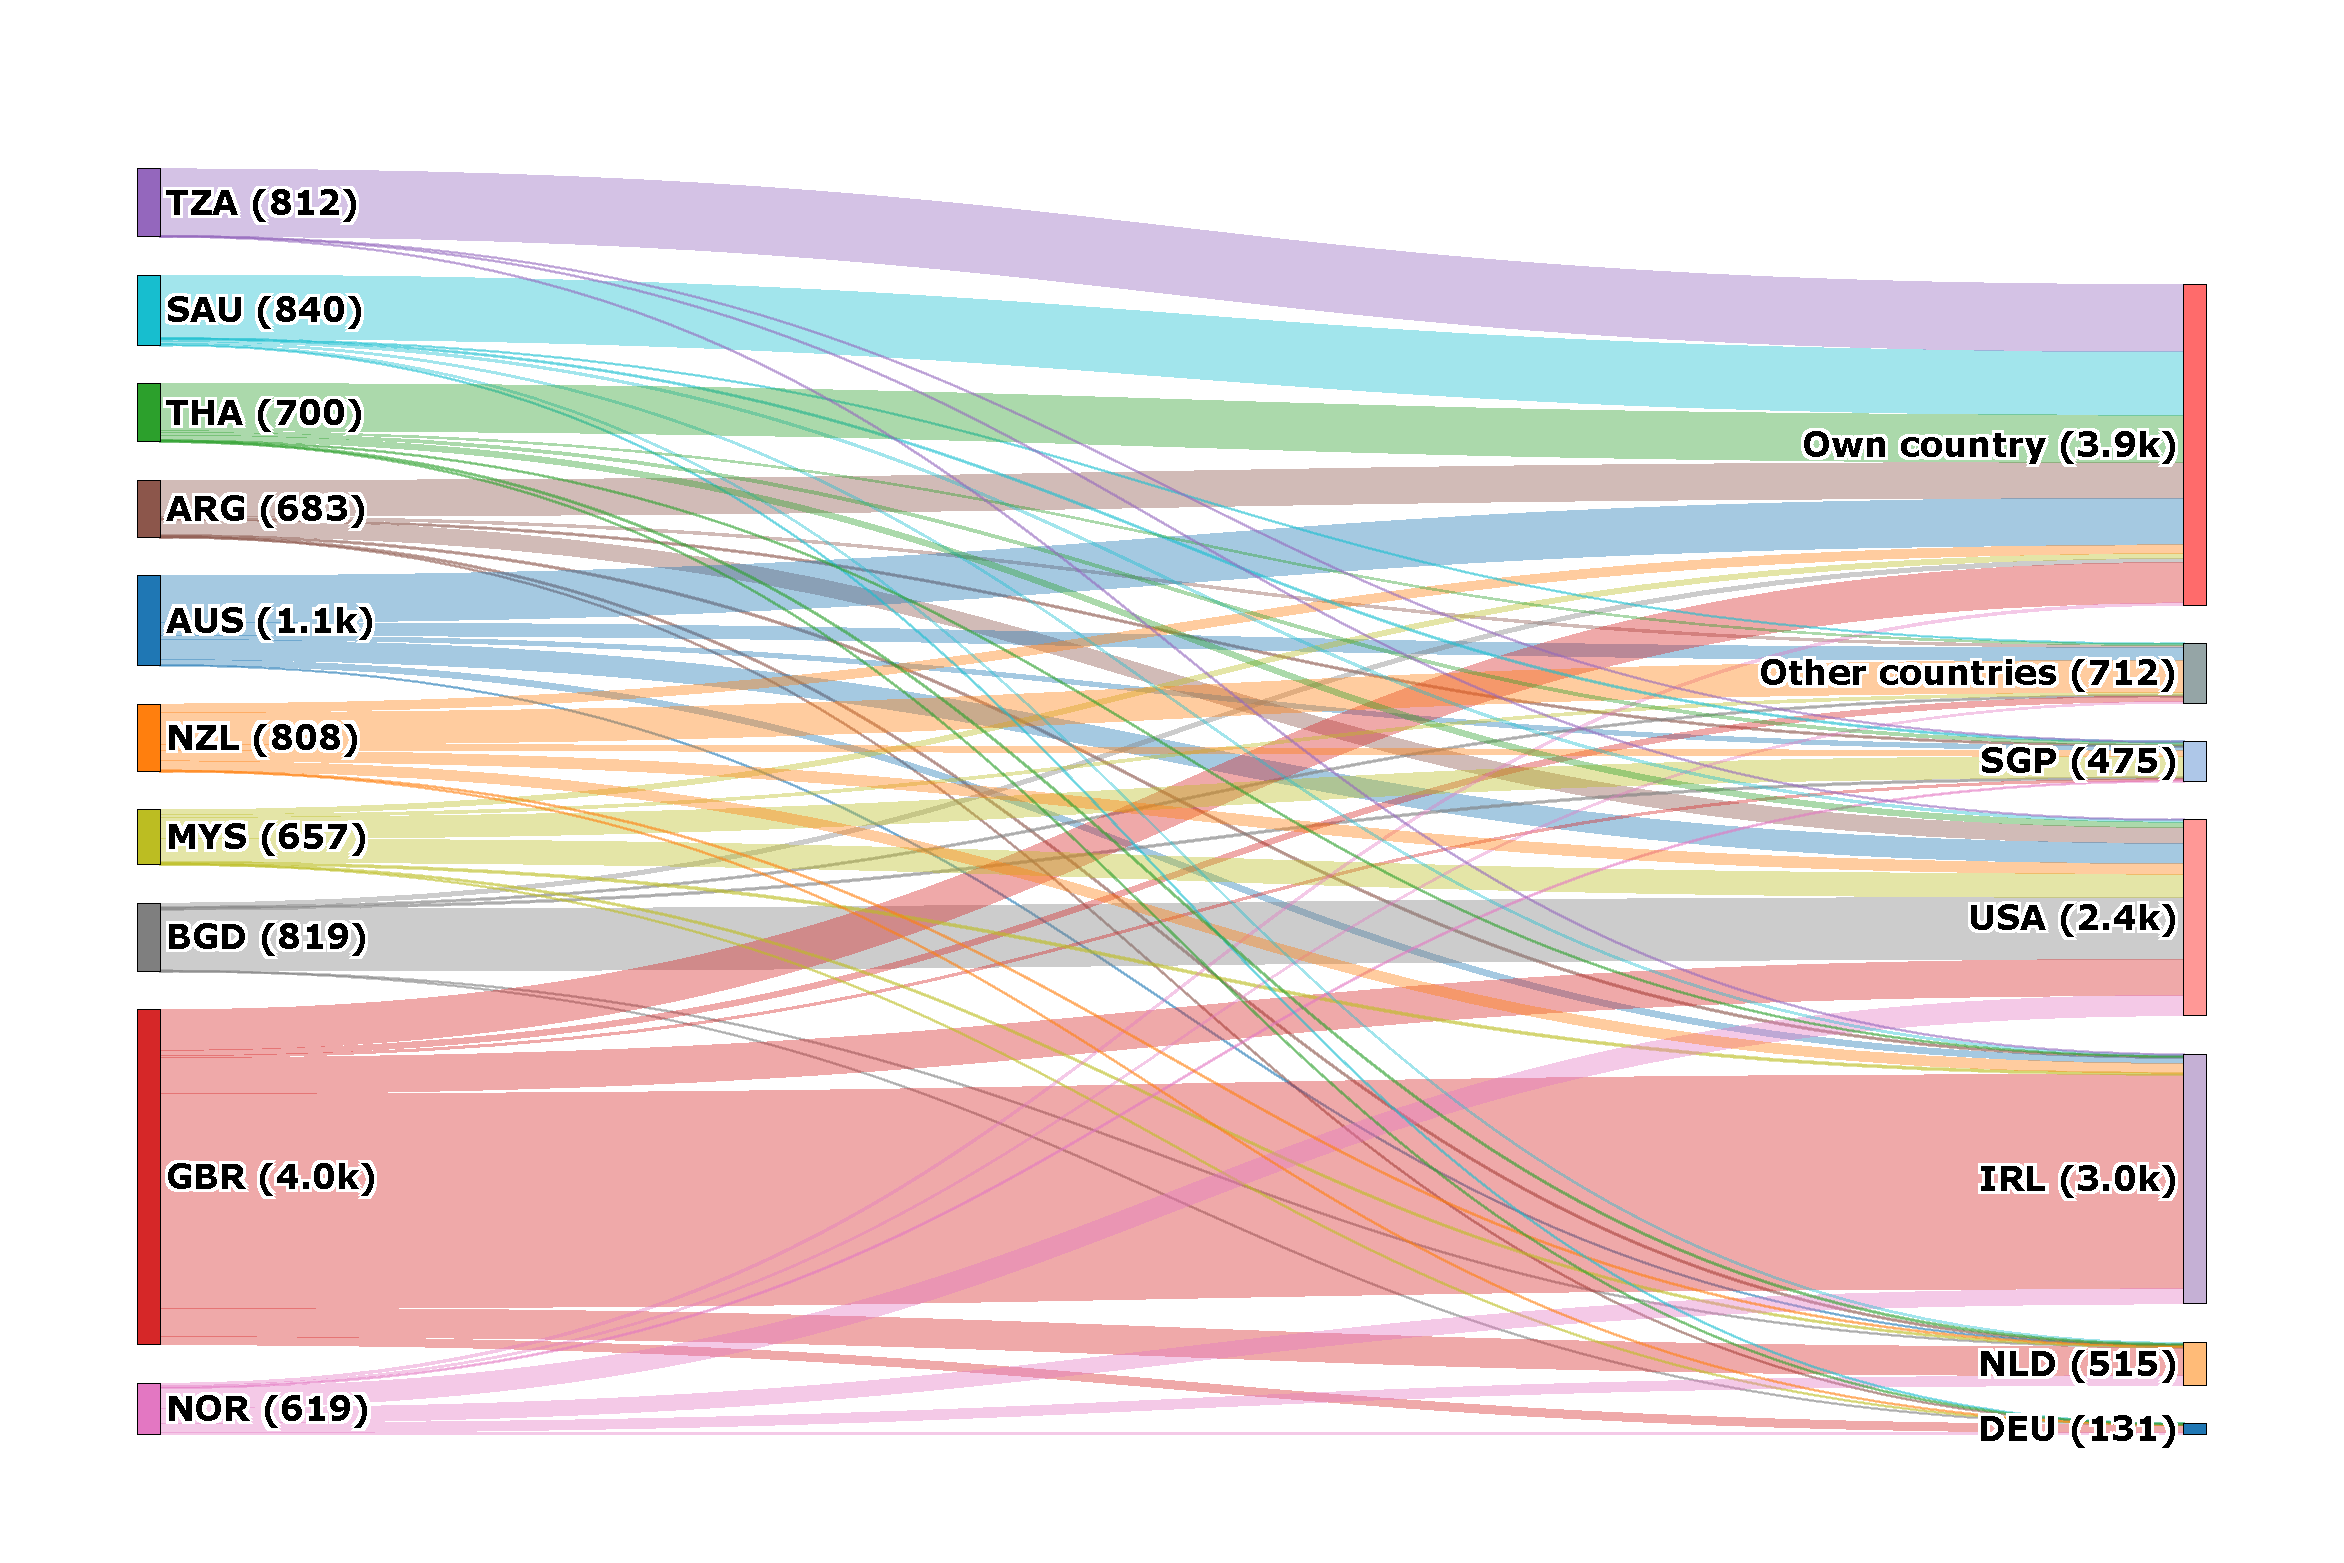
\includegraphics[width=\linewidth]{figures/gov_countryxcountry_sankey.pdf}
    \caption{DMARC data flow in governmental domains.}
    \label{fig:gov_countryxcountry_sankey}
    \vspace{-15px}
\end{figure}

\cref{fig:longitudinal_reporting_comb_analysis} shows a longitudinal analysis indicating which countries have \gls{DMARC} configured to send the most (in \%) \gls{DMARC} telemetry data to external domains.
%In other words, the \gls{ccTLD} of domain names with DMARC is different from the \gls{TLD} in \texttt{rua} and \texttt{ruf} tags. % repetition from the methodology.
We observe that Danish domains have the highest percentage of external reporting, starting from 27.4k (64.5\%) to 97.7k (82.7\%). However, in the last snapshot, we observe the use of \textit{robot.simply.com} on 51\% of its domains, which is a Danish hosting provider.
Denmark has the highest percentage, 79.5\% (128 cases most recently) of government domains sending \gls{DMARC} reports to foreign countries.
We observe a range of specialized email security companies, \eg Centera (Danish company, 65 instances), DMARCadvisor (Dutch company, 33 cases), and DMARCian (U.S. company, 14 cases).
Poland has the lowest use of external reporting: from 18.4k (9.2\%) to 34.7k (12.2\%), and governmental domains account for $\approx$4\% (around 15 instances throughout the period).
We also observe a recent increase in external reporting in Canada, the UK, Australia, and Brazil. In all cases, the top report destination configured is \textit{onsecureserver.net} from GoDaddy, with 105.7k (44.1\%), 233.3k (38.1\%), 101.3k (29.3\%), and 30.6k (12.2\%), respectively.
Our \dataset missed a few consecutive data points for Australia at the start of the 1.5-year period, we did not find Colombian's government domains from our data sources and France's government domain had only 1 internal reporter.

\begin{figure}[tb]
    \centering
    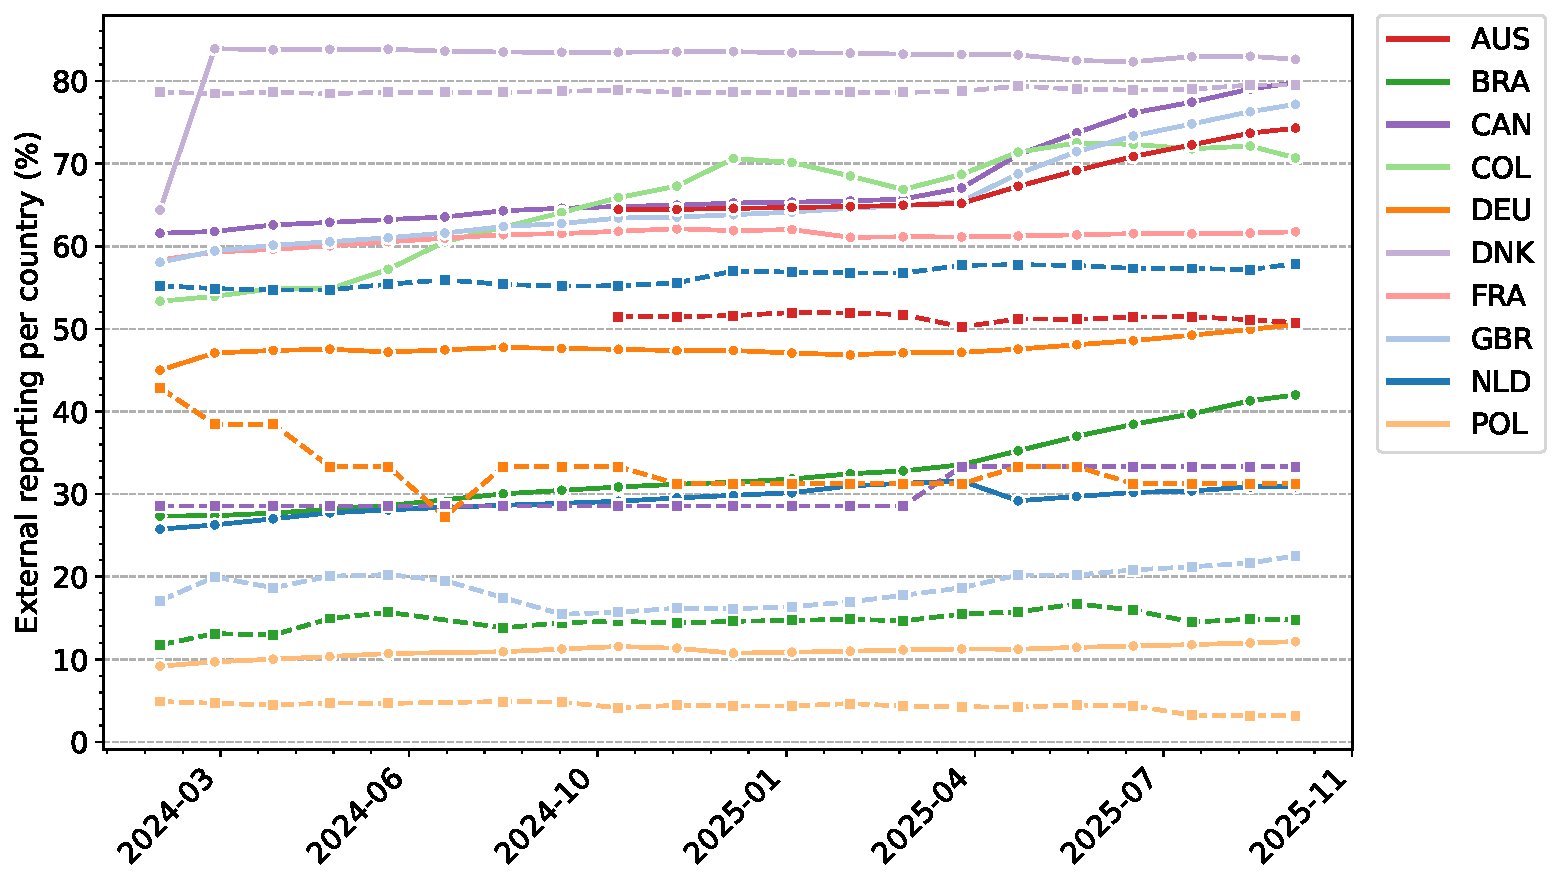
\includegraphics[width=1.\linewidth]{figures/longitudinal_reporting_comb_analysis.pdf}
    \caption{Countries that most use DMARC reporting from 2024-02 to 2025-10. Solid lines represent \gls{ccTLD} domains. Dashed lines represent governmental domains.}
    \label{fig:longitudinal_reporting_comb_analysis}
    \vspace{-15px}
\end{figure}
